
\documentclass[utf8]{article}
\usepackage[utf8]{inputenc}

\usepackage[parfill]{parskip}
\usepackage{booktabs}
\usepackage{amsmath}
\usepackage{amssymb}
\usepackage{amsfonts}
\usepackage{graphicx}
\usepackage{float}
\usepackage{listingsutf8}
\usepackage{listings}
\usepackage{graphicx}
\usepackage{hyperref}
\usepackage{fullpage}
\usepackage{lipsum}
\usepackage{multirow}

\nocite{*}
\setlength\parindent{24pt}

\begin{document}
\begin{titlepage}


  \author{Andrius Ezerskis \& Moïra Vanderslagmolen}
  \title{Projet d'Algorithmique: R-trees}

  \maketitle
\end{titlepage}
\tableofcontents
\newpage
\begin{large}



  \section{Introduction}
  \indent
  \par


  \par
  \section{RTree}
  \subsection{Création RTree}
  \par
  \indent
  Au début, nous avions N, le truc maximum pr les RTree en attribut de la classe RTree et défini là dedans.
  Pour optimiser notre programme, nous avons décidé de le passer en paramètre.
  Grâce à cette amélioration, les 8 tests que nous avons fait tourner ont pris
  4,429 secondes au total au lieu de 5,865 secondes.

  \subsection{Split Linéaire}

  \subsection{Split Quadratique}
  L'algorithme de split quadratique commence par appeler le pickSeeds quadratique afin d'obtenir deux noeuds qui, leurs aires sommées, 
  prennent plus de place que le Minimum Bounding Rectangle qui les entoure.
  \newline Ensuite, la méthode pickNext s'assure de choisir, pour chaque sous-noeud, la seed dont le MBR augmente le moins avec ce sous-noeud, et 
  le sous-noeud devient alors l'enfant de cette seed.
  \newline Pour finir, les deux splitSeeds obtenus via pickSeeds reçoivent comme parent le node (celui que l'on doit split) et, réciproquement, 
  le node reçoit les deux splitSeeds comme ses enfants. Le noeud a été divisé.



  \section{Structure du code}

  \par
  \subsection{MBRNode}
  \par
  \indent
  MBRNode représente les noeuds des R-Tree. Elle contient un label, un polygone,
  des enfants (sauf si c'est une feuille) et un parent (sauf si c'est la racine de
  l'arbre). Si le noeud n'est pas une feuille, alors son label sera "SplitSeed",
  car il regroupe plusieurs polygones.

  \subsection{RTreeLinear}\label{RTreeLinear}
  \par
  \indent
  RTreeLinear représente l'implémentation du R-Tree avec l'algorithme de split linéaire.
  \subsection{RTreeQuadratic}\label{RTreeQ}

  \subsection{RTree}
  \par
  \indent
  RTree est une classe abstraite. Elle permet de regrouper ensemble les méthodes
  communes à RTreeLinear et RTreeQuadratic, par exemple la
  recherche d'un noeud (searchNode), l'initialisation de la classe


  \subsection{FileLoader}
  \par
  \indent
  Cette classe permet de charger le fichier en mémoire. Nous avons implémenté
  cette classe afin de facilement changer la façon dont les fichiers sont chargés
  en mémoire.

  \section{Optimisations}
  \subsection{Multi-polygones}
  \par
  \indent
  Notre première optimisation se base sur les multi-polygones. En effet, comme
  expliqué dans les consignes du projet d'algorithmique, nous avons remarqué que
  des polygones très étendu comme la france (voir annexe, mettre un label)
  prenaient énormément de place. Nous avons donc décidé de séparer les
  multi-polygones en polygones et ça a donné (figure aprèsopti). Cela nous a
  permis de gagner quelques secondes lors des tests dont nous parlerons au
  chapitre 'Analyse des tests'.

  \subsection{Split}
  \par
  \indent
  Au début, nous copions l'entiereté du vecteur des enfants du node choisi pour
  split. Puis nous vidons ce vecteur et nous rajoutons les seeds choisies. Et puis
  seulement avec le vecteur copié nous ajoutions au fur et à mesure au seeds
  choisies. Nous nous sommes dit qu'on perdait bcp de temps à copier l'entiereté
  du vecteur, surtout sur des gros vecteurs.

  Nous avons donc changé l'ordre, d'abord nous appelons pickNext pour qu'il
  rajoute les enfants aux seeds, puis nous vidons le vecteur du node à spliter et
  rajoutons les splits seeds.

  Grâce à cette amélioration, les 8 tests que nous avons fait tourner ont pris
  5,865 secondes au total au lieu de 6,778 secondes.
  \par
  \subsection{PickSeeds quadratique}
  \par
  \indent
  Dans le pickSeeds quadratique, nous itérons à travers le vecteur d'enfants du node à
  split et nous prenons les deux noeuds les plus éloignés. Nous avons vite
  remarqué qu'il n'était pas nécéssaire de faire un double for en itérant chaque
  élément dans le vecteur. En effet, si nous calculons l'aire pour le noeud A
  et pour le noeud B, il ne faut pas recalculer pour le noeud B et le noeud A, de
  même qu'il ne faut pas calculer l'aire pour le noeud A et le noeud A. Nous
  faisons donc deux boucles for, l'une itérant dans le vecteur entier de
  sous-noeuds, l'autre commençant à l'indice de la précédente boucle + 1. De cette
  manière, nous commençons avec le noeud A et calculons avec le noeud B et tous
  les autres noeuds restants, puis le noeud B avec le noeud C et ainsi de suite.
  Cela nous permet de réduire le temps d'exécution.
  \par


  \section{Expérience sur données réelles}
  \subsection{Présentation des tests}
  \begin{enumerate}
    \item Carte de la belgique - Algorithme linéaire - Campus universitaire
    \item Carte de la belgique - Algorithme linéaire - Point pas dans le polygone
    \item Carte du monde - Algorithme linéaire - Kazakhstan
    \item Carte du monde - Algorithme linéaire - Canada
    \item Carte de la france - Algorithme linéaire - Auvergne
    \item Carte de la france - Algorithme linéaire - Guyane
    \item Carte de la belgique - Algorithme quadratique - Campus universitaire
    \item Carte de la belgique - Algorithme quadratique - Point pas dans le polygone
    \item Carte du monde - Algorithme quadratique - Kazakhstan
    \item Carte du monde - Algorithme quadratique - Canada
    \item Carte de la france - Algorithme quadratique - Auvergne
    \item Carte de la france - Algorithme quadratique - Guyane
  \end{enumerate}

  \subsection{Présentation des cartes}
  \begin{enumerate}
    \item Carte de la belgique : 19795 polygones
    \item Carte du monde : 251 polygones
    \item Carte de la france : 18 polygones
  \end{enumerate}




  \subsection{Résultats des tests}
  \par
  \indent
  Temps en millisecondes de la fonction search en fonction des différents tests et valeurs.

  \begin{tabular}{ |p{3cm}||p{3cm}|p{3cm}|p{3cm}|  }
    \hline
    \multicolumn{4}{|c|}{Temps en millisecondes de la fonction search} \\
    \hline
    Test   & N=4 & N = 500 & N = 10000                                 \\
    \hline
    Test1  & 15  & 15      & 17                                        \\
    Test2  & 1   & 1       & 1                                         \\
    Test3  & 76  & 8       & 11                                        \\
    Test4  & 123 & 214     & 219                                       \\
    Test5  & 23  & 68      & -                                         \\
    Test6  & 3   & 3       & -                                         \\
    Test7  & 2   & 0       & 2                                         \\
    Test8  & 1   & 1       & 4                                         \\
    Test9  & 3   & 2       & 2                                         \\
    Test10 & 29  & 76      & 73                                        \\
    Test11 & 29  & 37      & -                                         \\
    Test12 & 2   & 2       & -                                         \\
    \hline
  \end{tabular}

  \begin{tabular}{ |p{3cm}||p{3cm}|p{3cm}|p{3cm}|  }
    \hline
    \multicolumn{4}{|c|}{Temps en millisecondes de la fonction search avec l'optimisation} \\
    \hline
    Test   & N=4 & N = 500 & N = 10000                                                     \\
    \hline
    Test1  & 12  & 14      & 19                                                            \\
    Test2  & 1   & 1       & 6                                                             \\
    Test3  & 11  & 12      & 9                                                             \\
    Test4  & 20  & 28      & 23                                                            \\
    Test5  & 99  & 95      & -                                                             \\
    Test6  & 3   & 2       & -                                                             \\
    Test7  & 3   & 0       & 2                                                             \\
    Test8  & 0   & 3       & 2                                                             \\
    Test9  & 1   & 2       & 2                                                             \\
    Test10 & 5   & 5       & 6                                                             \\
    Test11 & 29  & 19      & -                                                             \\
    Test12 & 2   & 2       & -                                                             \\
    \hline
  \end{tabular}



  \subsection{Analyse des données}
  \subsubsection{Optimisation}
  \par
  \indent
  Nous avons donc remarqué suite à cela que le test 4 prenait beaucoup de temps,
  et plus généralement les tests concernant la carte du monde (Test 3, 4, 9, 10)
  et les tests concernant la carte de la france (Test 5,6,11,12). Ces tests
  devraient être les plus rapides, car ils contiennent le moins de polygones, et
  les algorithmes sont quadratiques et linéaire. Nous avons compris que le
  problème venait du fait que les multi-polygones prenait énormément de place et nous avons refait les tests
  \subsubsection{Influence du N}
  Nous remarquons aussi que le
  nombre N n'a pas d'influence sur la rapidité de notre algorithme.
  \subsubsection{Algorithme linéaire vs Algorithme quadratique}
  \par
  \indent
  Nous avons aussi remarqué que l'algorithme linéaire prend beaucoup plus de temps
  à chercher un point dans un polygone. En moyenne, la recherche prend 39,9
  millisecondes pour l'algorithme linéaire et 13,25 millisecondes pour
  l'algorithme quadratique. Nous avons donc comparé les temps d'exécution. En
  moyenne, le temps d'exécution sur 6 tests pour l'algorithme quadratique est de
  6,357 secondes. Le temps d'exécution sur les mêmes tests pour l'algorithme
  linéaire est de 3,087 secondes. La création de l'arbre est donc beaucoup plus
  rapide pour l'algorithme linéaire que pour le quadratique, ce qui est attendu vu
  la complexité de chaque algorithme. Cependant, il est intéressant de noter que
  la fonction de recherche prend beaucoup plus de temps dans l'algorithme
  linéaire.
  \par

  \section{Conclusion}
  \indent
  \par
  \par

  \section{Bibliographie}

  \section{Annexes}
  \begin{figure}[h]
    \caption{Before optimization}
    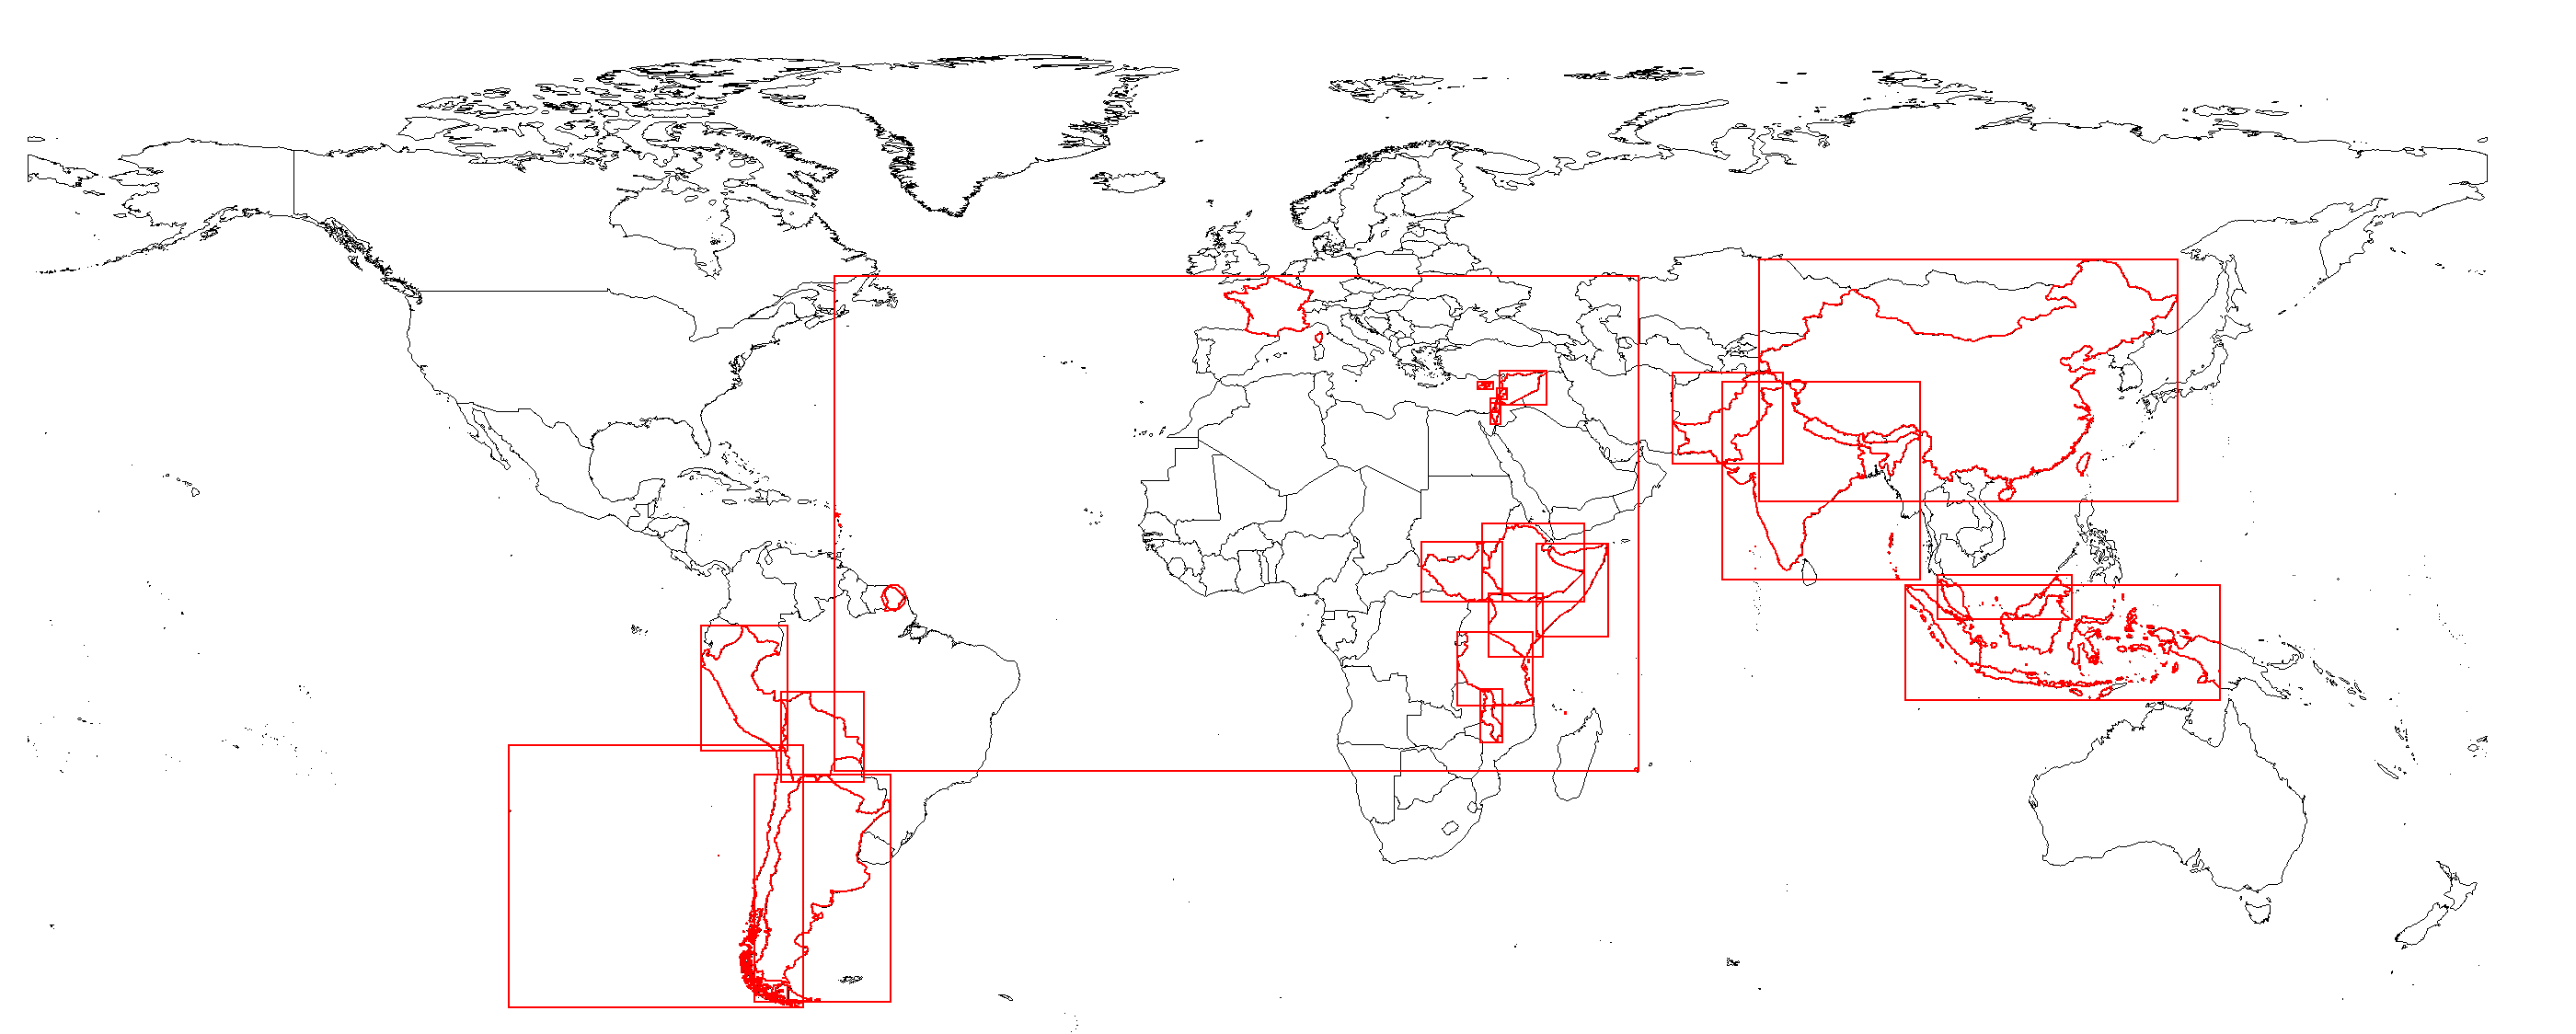
\includegraphics[width=\textwidth]{beforeopti.png}\label{fig:beforeopti}
  \end{figure}

  \begin{figure}[h]
    \caption{After optimization}
    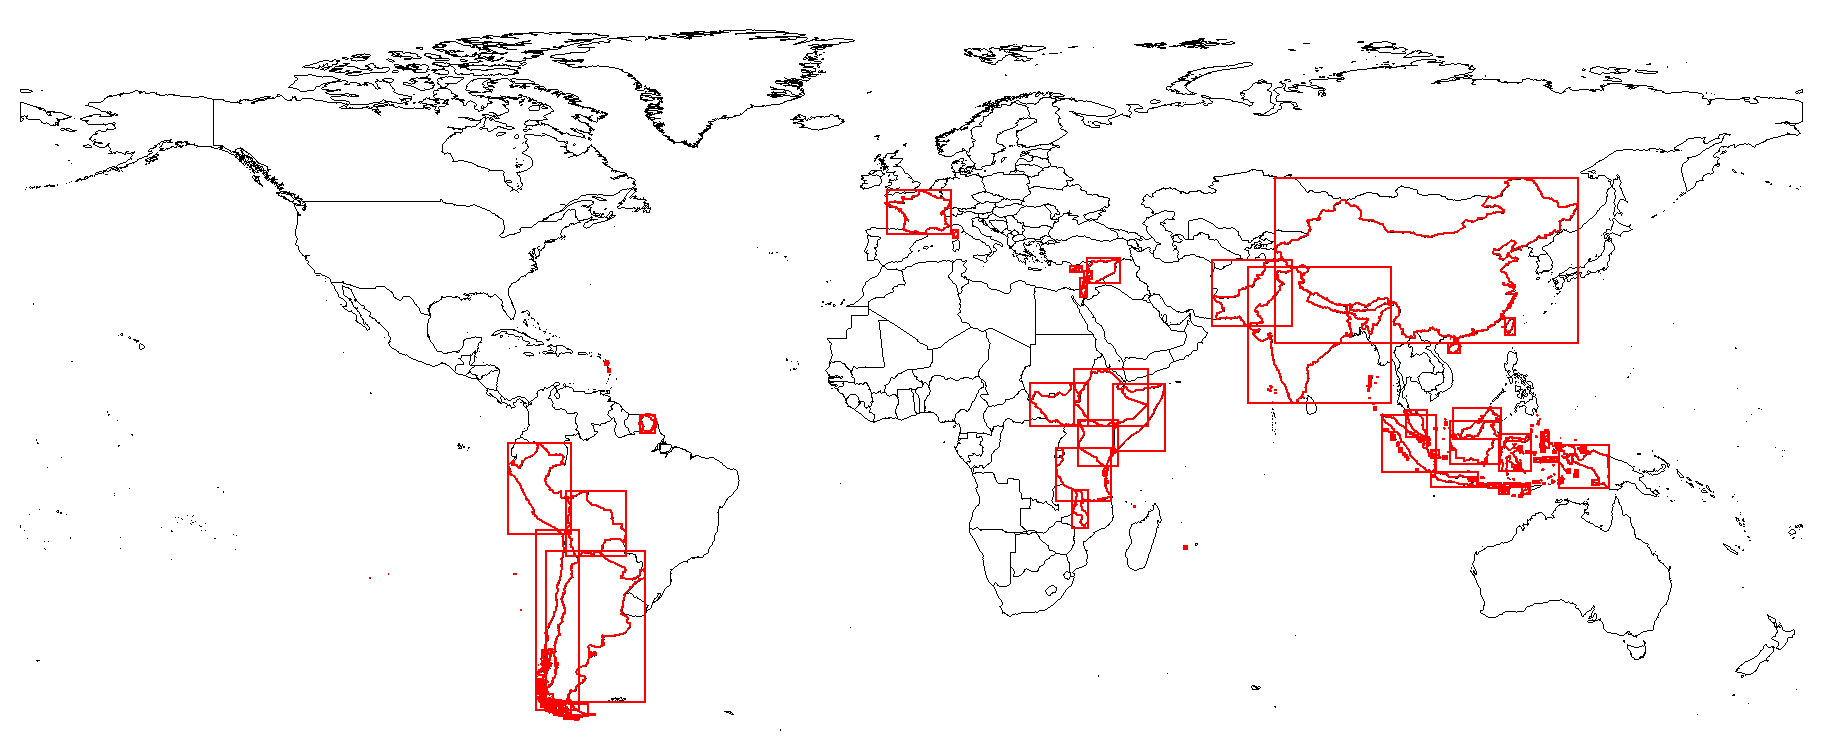
\includegraphics[width=\textwidth]{afterOpti.png}\label{fig:afteropti}
  \end{figure}


\end{large}

\end{document}
